\documentclass{beamer}

\usetheme{Darmstadt}
\usefonttheme[onlylarge]{structurebold}
\setbeamerfont*{frametitle}{size=\normalsize,series=\bfseries}
\setbeamertemplate{navigation symbols}{}

% Standard packages

\usepackage[english]{babel}
\usepackage[latin1]{inputenc}
\usepackage{times}
\usepackage[T1]{fontenc}
\usepackage{float}
\usepackage{graphicx}
\usepackage{subcaption}
\usepackage{ifthen}
\usepackage{minted}
\usepackage{verbatim}
%\usepackage{multimedia}
\usepackage{movie15}

% Setup TikZ
\usepackage{tikz}
\usetikzlibrary{arrows}
\tikzstyle{block}=[draw opacity=0.7,line width=1.4cm]


% Author, Title, etc.
\title[Pure functional programming in Agent-Based Simulation] 
{%
  Pure functional programming \\ in Agent-Based Simulation
}

\author[Thaler]
{
  Jonathan~Thaler
}

\institute[University of Nottingham, Ningbo, China]
{
  University of Nottingham, Ningbo, China
}

\date[AIOP Seminar 2019]
{AIOP Seminar 2019}

% The main document
\begin{document}

\begin{frame}
  \titlepage
\end{frame}

\section{Introduction}
\begin{frame}{The Metaphor}
\begin{itemize}
  \item "[..] object-oriented programming is a particularly natural development environment for Sugarscape specifically and artificial societies generally [..]" (Epstein et al 1996)
  
  \item "agents map naturally to objects" (North et al 2007)
\end{itemize}
\end{frame}

\begin{frame}{Outline}
\begin{itemize}
  \item What is Agent-Based Simulation (ABS)?
  
  \item What is \textit{pure} Functional Programming (FP)?
  
  \item How can we do ABS + FP?  
  
  \item ABS + FP = ?
  
  \item Conclusions
\end{itemize}
\end{frame}

\section{Agent-Based Simulation}
\begin{frame}{What is Agent-Based Simulation (ABS)?} 
  \begin{block}{Example}
    \textit{\textbf{Simulate} the spread of an infectious disease in a city. \\ What are the \textbf{dynamics} (peak, duration of disease)?}
  \end{block}
  
  \begin{enumerate}
    \item Start with population \, \, \, \, \, \, \, $\to$ Agents
 	\item Situated in City \, \, \, \, \, \, \, \, \, \, \, \,\, $\to$ Environment
 	\item Interacting with each other \, $\to$ Local interactions
 	\item Creating dynamics \, \, \, \, \, \, \, \,\,\, $\to$ Emergent system behaviour
 	\item Therefore ABS \, \, \, \, \, \, \, \, \, \, \, \,\,\, $\to$ Bottom-up approach
  \end{enumerate}
\end{frame}

\begin{frame}{SIR Model}
  
\includegraphics[width=0.7\textwidth]{./fig/SIR_transitions.png}
  
  \begin{itemize}
    \item Population size $N = 1,000$
 	\item Contact rate $\beta = 5$
 	\item Infection probability $\gamma = 0.05$
 	\item Illness duration $\delta = 15$
 	\item 1 initially infected agent
  \end{itemize}
    
  \begin{block}{System Dynamics}
    Top-Down, formalised using Differential Equations, give rise to dynamics.
  \end{block}
\end{frame}

\begin{frame}{SIR Model Dynamics}
  \center
  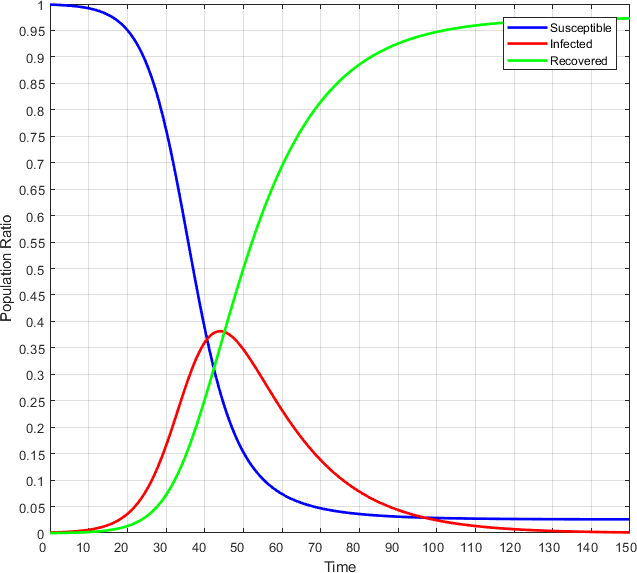
\includegraphics[width=0.7\textwidth]{./fig/SIR_SD_001dt.png}
\end{frame}

\begin{frame}[fragile]{Defining Spatiality}
\begin{figure}
\begin{center}

\includegraphics[width=0.2\textwidth]{./fig/moore.png}
\caption*{Moore Neighbourhood}
\end{center}
\end{figure}
\end{frame}

\begin{frame}{Spatial Dynamics}
\begin{figure}
\begin{center}
	\begin{tabular}{c c}
		\begin{subfigure}[b]{0.4\textwidth}
			\centering
			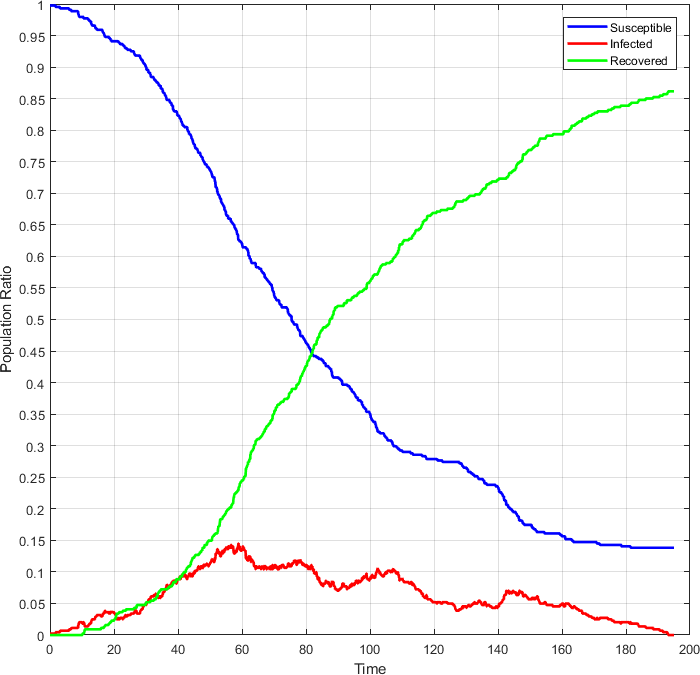
\includegraphics[width=0.95\textwidth, angle=0]{./fig/SIR_Dunai_dt001.png}
			\caption*{Agent-Based}
		\end{subfigure}
    	
    	&
  
		\begin{subfigure}[b]{0.4\textwidth}
			\centering
			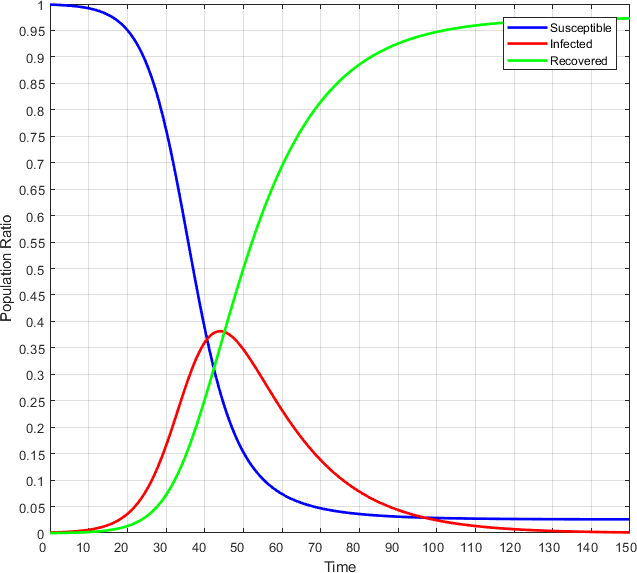
\includegraphics[width=1\textwidth, angle=0]{./fig/SIR_SD_001dt.png}
			\caption*{System Dynamics}
		\end{subfigure}
	\end{tabular}
\end{center}
\end{figure}
\end{frame}

\begin{frame}{Spatial Visualisation}
%\movie[width=10cm,height=5.5cm]{Dynamics 21x21 2D Environment}{./video/SIR_DUNAI_dt001.mp4}
\includemovie[rate=2]{11cm}{6.5cm}{./video/SIR_DUNAI_dt001.mp4}
\end{frame}

\section{Pure functional programming}
\begin{frame}[fragile]{What is pure functional programming?}
  \begin{block}{Functions as first class citizens}
  	Passed as arguments, returned as values and assigned to variables.
  \end{block}
  
  \begin{block}{}
  \begin{minted}[fontsize=\normalsize]{haskell}
  map :: (a -> b) -> [a] -> [b]
	
  const :: a -> (b -> a)
  const a = (\_ -> a)
  \end{minted}
  \end{block}
\end{frame}
 
\begin{frame}[fragile]{What is pure functional programming cont'd?}
  \begin{block}{Immutable data}
 	Variables can not change, functions return new copy. \\ Data-Flow oriented programming.
  \end{block}
  
  \begin{block}{}
  \begin{minted}[fontsize=\normalsize]{haskell}
  let x   = [1..10]
      x'  = drop 5 x
      x'' = x' ++ [10..20] 
  \end{minted}
  \end{block}
\end{frame}
 
\begin{frame}[fragile]{What is pure functional programming cont'd?}
  \begin{block}{Recursion}
 	To iterate over and change data. 
  \end{block}
  
  \begin{block}{}
  \begin{minted}[fontsize=\normalsize]{haskell}
  fact :: Int -> Int
  fact 0 = 1
  fact n = n * fact (n-1)
  \end{minted}
  \end{block}
\end{frame}
 
\begin{frame}[fragile]{What is pure functional programming cont'd?}
  \begin{block}{Declarative style}
  	Describe \textit{what} to compute instead of \textit{how}.
  \end{block}
  
  \begin{block}{}
  \begin{minted}[fontsize=\normalsize]{haskell}
  mean :: [Double] -> Double
  mean xs = sum xs / length xs
  \end{minted}
  \end{block}
\end{frame}
 
\begin{frame}[fragile]{What is pure functional programming cont'd?}
  \begin{block}{Explicit about Side-Effects}
  	Distinguish between side-effects of a function \textit{in its type}.
  \end{block}
  
  \begin{block}{}
  \begin{minted}[fontsize=\normalsize]{haskell}
  readFromFile :: String -> IO String
  randomExponential :: Double -> Rand Double
  statefulAlgorihm :: State Int (Maybe Double)
  produceData :: Writer [Double] ()
  \end{minted}
  \end{block}
\end{frame}

\section{ABS + FP}
\begin{frame}{How can we do ABS + FP?}
  \begin{block}{How can we represent an Agent, its local state and its interface?}
	We don't have objects and mutable state...
  \end{block}
  
  \begin{block}{How can we implement direct agent-to-agent interactions?}
	We don't have method calls and mutable state...
  \end{block}
  
  \begin{block}{How can we implement an environment and agent-to-environment interactions?}
	We don't have method calls and mutable state...
  \end{block}
  
  \begin{block}{Solution}
  	Functional Reactive Programming with Monadic Stream Functions
  \end{block}
\end{frame}

\begin{frame}{Arrowized Functional Reactive Programming (AFRP)}
  \begin{itemize}
    \item Continuous- \& discrete-time systems in FP
 	\item Signal Function 
 	\item Events
 	\item Effects like random-numbers, global state, concurrency
 	\item \textit{Arrowized} FRP using the \textit{Dunai} library
  \end{itemize}
\end{frame}

\begin{frame}{Monadic Stream Functions (MSF)}
  \begin{block}{Process over time}
  \begin{flalign*}
	SF \, \alpha \, \beta \approx Signal \, \alpha \rightarrow Signal \, \beta \\
	Signal \, \alpha \approx Time \rightarrow \alpha 
  \end{flalign*}
  \end{block}
  
  \begin{block}{Agents as Signal Functions}
  \begin{itemize}
  	\item Clean interface (input / output)
  	\item Pro-activity by perceiving time
  \end{itemize}
  \end{block}
\end{frame}

\begin{frame}[fragile]{Arrowized Functional Reactive Programming (AFRP)}
\begin{block}{}
\begin{minted}[fontsize=\footnotesize]{haskell}
type AgentId    = Int
data Message    = Tick Int | MatingRequest AgentGender ... 
data AgentState = AgentState { agentAge :: Int, ... }             
data Observable = Observable { agentAgeObs :: Int, ... } 
data AgentOut   = AgentOut
  { kill       :: Bool
  , observable :: Observable
  , messages   :: [(AgentId, Message)] -- list of messages with receiver
  }
-- agent continuation has different types for input and output
newtype AgentCont inp out = AgentCont (inp -> (out, AgentCont inp out))
-- taking the initial AgentState as input and returns the continuation
sugarscapeAgent :: AgentState -> AgentCont (AgentId, Message) AgentOut
sugarscapeAgent asInit = AgentCont (\ (sender, msg) -> 
  case msg of
    agentCont (sender, Tick t) = ... handle tick
    agentCont (sender, MatingRequest otherGender) = ... handle mating request)
\end{minted}
\end{block}
\end{frame}

\section{ABS + FP = ?}
\begin{frame}{ABS + FP = Type Saftey}
	\begin{block}{Epstein et al (1996)}
    "... when the sequence of random numbers is specified ex ante the model is deterministic. Stated yet another way, model output is invariant from run to run when all aspects of the model are kept constant including the stream of random numbers."
    \end{block}
    
  \begin{itemize}
  	%\item Can guarantee that in our pure functional approach already at compile time.
    \item Purity guarantees reproducibility.
    \item Enforce and guarantee update semantics.
  \end{itemize}
\end{frame}

\begin{frame}{ABS + FP = Software Transactional Memory}
  \begin{itemize}
    \item Concurrency using Software Transactional Memory (STM)
    \item Lock free!
    \item Tremendous performance improvement
    \item Substantially outperforms lock-based implementation 
    \item STM semantics retain guarantees about non-determinism
  \end{itemize}
\end{frame}

\begin{frame}{ABS + FP = Software Transactional Memory cont'd}
  \begin{itemize}
    \item With Haskell typesystem can be explicit in side-effects: STM only
    \item Guarantees that the non-determinism comes only from concurrency within STM and nothing else
  \end{itemize}
\end{frame}

\begin{frame}{ABS + FP = Property-Based Testing}
  \begin{itemize}
    \item Express specifications directly in code and generate random test cases
    \item Stochastic nature of Property-Based TEsting and ABS should be perfect match
  \end{itemize}
\end{frame}

\begin{frame}{ABS + FP = Property-Based Testing cont'd}
  \begin{itemize}
    \item Express specifications directly in code and generate random test cases
    \item Stochastic nature of Property-Based TEsting and ABS should be perfect match
  \end{itemize}
\end{frame}

\section{Conclusion}
\begin{frame}{Conclusion}
  \begin{itemize}
    \item The direction is towards an simulation which is more likely to be correct with the ultimate goal being a correct-by-construction implementation (up to some specification).
    \item A correct-by-construction implementation does NOT relief us from actually running the simulation!
    \item 
  \end{itemize}
\end{frame}

\begin{frame}{}
  \begin{center}
  Thank You!
  \end{center}
\end{frame}
\end{document}